	\makeatletter
	\def\@makechapterhead#1{%
	  \vspace*{50\p@}%
	  {\parindent \z@ \centering\normalfont
	    \ifnum \c@secnumdepth >\m@ne
	      \if@mainmatter
	         \Large\bfseries \@chapapp\space \thechapter
 	        \par\nobreak
	        \vskip 20\p@
	      \fi
	    \fi
	    \interlinepenalty\@M
	     \Large \bfseries #1\par\nobreak
	
	    \vskip 40\p@
	  }}
	\def\@makeschapterhead#1{%
	  \vspace*{50\p@}%
	  {\parindent \z@ \centering 
	    \normalfont
	    \interlinepenalty\@M
	    \Large\bfseries  #1\par\nobreak
	    \vskip 40\p@
	  }}
	\makeatother
	\titlespacing*{\chapter}{0pt}{0pt}{12pt}
\chapter{Testing}

\section{General}
The purpose of testing is to discover errors. Testing is the process of trying to discover every conceivable fault or weakness in a work product. It provides a way to check the functionality of components, sub assemblies, assemblies and/or a finished product. It is the process of exercising software with the intent of ensuring that the Software system meets its requirements and user expectations and does not fail in an unacceptable manner. There are various types of test. Each test type addresses a specific testing requirement.

\section{Developing Methodologies}
The test process is initiated by developing a comprehensive plan to test the general functionality and special features on a variety of platform combinations. Strict quality control procedures are used.The process verifies that the application meets the requirements specified in the system requirements document and is bug free. The following are the considerations used to develop the framework from developing the testing methodologies


\section{Robotium  benefits over other }

\begin{figure} [ht]
\centering

\includegraphics[scale=0.5]{robotinium}\\
\caption{Robotinium Automatic Application Testing Package }
\label{the-label-for-cross-referencing}
\end{figure}

\begin{itemize}
 \item You can develop powerful test cases, with minimal knowledge of the application under test.
 \item The framework handles multiple Android activities automatically.
 \item  Minimal time needed to write solid test cases.
 \item  Readability of test cases is greatly improved, compared to standard instrumentation tests.
 \item ] Test cases are more robust due to the run-time binding to GUI components.
 \item Blazing fast test case execution.
 \item Integrates smoothly with Maven or Ant to run tests as part of continuous integration.
\end{itemize}

\section{Results}
\begin{figure} [ht]
\centering
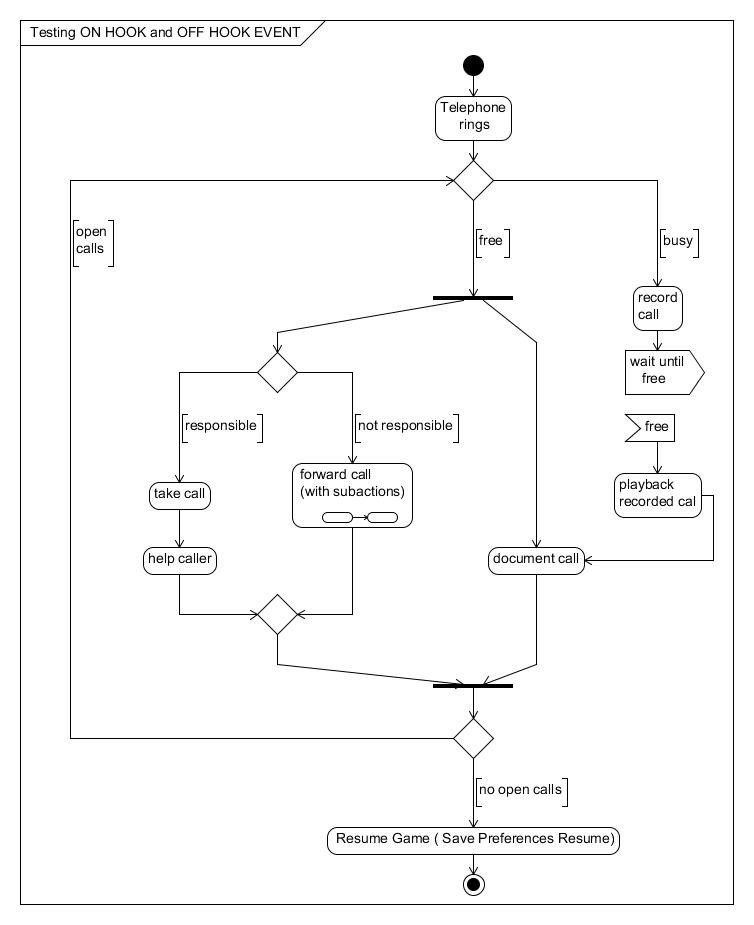
\includegraphics[scale=0.5]{testingcall}\\
\caption{Testing ON and OFF HOOK  }
\label{the-label-for-cross-referencing}
\end{figure}

\subsection{Analysis}
Code Snippet
\lstinputlisting{robotinium.py}

